% ------------------------------------------------------------
% Tool Hub — Tai lieu ky thuat du an
% Bien dich: xelatex tool-hub-documentation.tex
% ------------------------------------------------------------
\documentclass[12pt,a4paper]{article}

% === Packages ===
\usepackage[margin=2.2cm]{geometry}
\usepackage{xcolor}
\usepackage{fontspec}
\usepackage{titlesec}
\usepackage{fancyhdr}
\setlength{\headheight}{13.59999pt}
\usepackage{hyperref}
\usepackage{listings}
\usepackage{graphicx}
\usepackage{parskip}
\usepackage{booktabs}
\usepackage{tabularx}
\usepackage{enumitem}
\usepackage{tikz}
\usetikzlibrary{arrows.meta, positioning, shapes.geometric}

% === Font ===
\setmainfont{DejaVu Serif}
\setsansfont{DejaVu Sans}
\setmonofont{DejaVu Sans Mono}

% === Colors ===
\definecolor{primary}{HTML}{1a56db}
\definecolor{secondary}{HTML}{059669}
\definecolor{dark}{HTML}{111827}
\definecolor{graytext}{HTML}{6b7280}
\definecolor{codebg}{HTML}{f3f4f6}
\definecolor{codeborder}{HTML}{d1d5db}

% === Hyperlinks ===
\hypersetup{
  colorlinks=true,
  linkcolor=primary,
  urlcolor=primary,
  citecolor=primary,
}

% === Code listing style (Python) ===
\lstdefinestyle{py}{
  language=Python,
  backgroundcolor=\color{codebg},
  basicstyle=\small\ttfamily,
  keywordstyle=\color{primary}\bfseries,
  commentstyle=\color{graytext}\itshape,
  stringstyle=\color{secondary},
  numberstyle=\tiny\color{graytext},
  numbers=left,
  numbersep=5pt,
  frame=single,
  rulecolor=\color{codeborder},
  breaklines=true,
  tabsize=4,
  showstringspaces=false,
}

% === Code listing style (TypeScript / Vue) ===
\lstdefinestyle{ts}{
  language=Python,
  backgroundcolor=\color{codebg},
  basicstyle=\small\ttfamily,
  keywordstyle=\color{primary}\bfseries,
  commentstyle=\color{graytext}\itshape,
  stringstyle=\color{secondary},
  numberstyle=\tiny\color{graytext},
  numbers=left,
  numbersep=5pt,
  frame=single,
  rulecolor=\color{codeborder},
  breaklines=true,
  tabsize=2,
  showstringspaces=false,
}

% === Code listing style (bash / Docker) ===
\lstdefinestyle{bash}{
  language=bash,
  backgroundcolor=\color{codebg},
  basicstyle=\small\ttfamily,
  keywordstyle=\color{primary}\bfseries,
  commentstyle=\color{graytext}\itshape,
  numberstyle=\tiny\color{graytext},
  numbers=left,
  numbersep=5pt,
  frame=single,
  rulecolor=\color{codeborder},
  breaklines=true,
  tabsize=2,
  showstringspaces=false,
}

% === Section formatting ===
\titleformat{\section}{\Large\bfseries\color{primary}}{}{0em}{}[\vspace{-0.3em}\rule{\textwidth}{0.5pt}]
\titleformat{\subsection}{\large\bfseries\color{dark}}{}{0em}{}
\titleformat{\subsubsection}{\normalsize\bfseries\color{secondary}}{}{0em}{}

% === Header / Footer ===
\pagestyle{fancy}
\fancyhf{}
\fancyhead[L]{\small\color{graytext} Tool Hub}
\fancyhead[R]{\small\color{graytext} Tai lieu ky thuat}
\fancyfoot[C]{\thepage}
\renewcommand{\headrulewidth}{0.4pt}

\begin{document}

% ============================================================
%  TITLE PAGE
% ============================================================
\begin{titlepage}
\centering
\vspace*{6em}
{\Huge\bfseries\color{primary} Tool Hub}\\[1em]
{\Large Hybrid Architecture --- FastAPI + NuxtUI + LangChain + Ollama}\\[2em]
{\large\color{graytext} Tai lieu ky thuat du an}\\[1em]
{\large\color{graytext} Phien ban 1.0}\\[3em]

\rule{0.6\textwidth}{0.5pt}\\[2em]

\begin{tabular}{ll}
\bfseries Sinh vien: & Phan Huu Binh Nguyen \\
\bfseries Ma so:     & 2403700211 \\
\bfseries Cong nghe: & FastAPI, NuxtUI/Vue 3, LangChain, Ollama/Qwen3 \\
\bfseries Trien khai: & Docker Compose (local), Vercel + Render (cloud) \\
\end{tabular}

\vfill
{\small\color{graytext} Ngay: \today}
\end{titlepage}

% ============================================================
%  TABLE OF CONTENTS
% ============================================================
\tableofcontents
\newpage

% ============================================================
%  1. TONG QUAN DU AN
% ============================================================
\section{Tong quan du an}

\subsection{Mo ta}

Tool Hub la mot he thong web tich hop nhieu cong cu phan tich du lieu (tools)
duoi dang plugin, duoc xay dung theo kien truc hybrid. Tool dau tien trong he
thong la Data Analytics Agent --- mot agent thong minh su dung mo hinh ngon ngu
lon (LLM) de phan tich du lieu tu file CSV, dua ra thong ke, bieu do, va bao
cao tu nhien.

\subsection{Muc tieu}

\begin{itemize}
  \item Xay dung mot Tool Hub co kha nang mo rong bang co che plugin (decorator).
  \item Tich hop agent phan tich du lieu voi 6 cong cu chuyen sau.
  \item Ho tro da bang (multi-table) --- agent co the lam viec voi nhieu file
        CSV trong cung mot du an.
  \item Hoi dap bang ca tieng Viet va tieng Anh.
  \item Trien khai bang Docker Compose (local) hoac Vercel + Render (cloud).
\end{itemize}

\subsection{Cong nghe chinh}

\begin{itemize}
  \item \textbf{FastAPI} --- Backend REST API (Python 3.12).
  \item \textbf{NuxtUI / Vue 3} --- Frontend SPA (Node 20).
  \item \textbf{LangChain 0.3} --- Agent orchestration, ReAct loop.
  \item \textbf{Ollama + Qwen3:1.7b} --- LLM inference (CPU).
  \item \textbf{Pandas + Plotly} --- Xu ly du lieu va ve bieu do.
  \item \textbf{ECharts (Vue-ECharts)} --- Hien thi bieu do o frontend.
  \item \textbf{Docker Compose} --- Dong goi 3 dich vu.
\end{itemize}

% ============================================================
%  2. CAU TRUC THU MUC
% ============================================================
\section{Cau truc thu muc}

\subsection{So do cay}

Duoi day la cau truc day du cua du an (chi bao gom file nguon, loai bo
\lstinline{node\_modules}, \lstinline{.nuft}, \lstinline{.output}, va
\lstinline{\_\_pycache\_\_}):

\small
\begin{lstlisting}[style=bash, language={}]
tool-hub/
├── .gitignore
├── README.md
├── docker-compose.yml
├── render.yaml
├── vercel.json
│
├── ollama/
│   ├── Dockerfile
│   └── entrypoint.sh
│
├── backend/
│   ├── .dockerignore
│   ├── .env
│   ├── Dockerfile
│   ├── requirements.txt
│   ├── sample_data/
│   │   └── sales_sample.csv
│   └── app/
│       ├── __init__.py
│       ├── config.py
│       ├── main.py
│       ├── core/
│       │   ├── __init__.py
│       │   └── registry.py
│       ├── tools/
│       │   ├── __init__.py
│       │   ├── tool_template/
│       │   │   ├── __init__.py
│       │   │   └── router.py
│       │   └── data_analytics/
│       │       ├── __init__.py
│       │       ├── router.py
│       │       ├── schemas.py
│       │       ├── project_manager.py
│       │       ├── agent/
│       │       │   ├── __init__.py
│       │       │   ├── analyst.py
│       │       │   └── prompts.py
│       │       └── analyst_tools/
│       │           ├── __init__.py
│       │           ├── chart_generator.py
│       │           ├── csv_reader.py
│       │           ├── query_data.py
│       │           └── statistics.py
│       └── uploads/
│           └── .gitkeep
│
└── frontend/
    ├── .dockerignore
    ├── Dockerfile
    ├── nuxt.config.ts
    ├── package.json
    ├── tsconfig.json
    ├── app.vue
    ├── layouts/
    │   └── default.vue
    ├── pages/
    │   ├── index.vue
    │   └── tools/
    │       └── data-analytics.vue
    ├── composables/
    │   └── useApi.ts
    ├── components/
    │   ├── hub/
    │   │   ├── Sidebar.vue
    │   │   └── ToolCard.vue
    │   └── data-analytics/
    │       ├── ChartView.vue
    │       ├── FileUpload.vue
    │       ├── LLMReport.vue
    │       ├── MultiFileUpload.vue
    │       ├── ProjectPanel.vue
    │       ├── StatsTable.vue
    │       └── TableList.vue
    └── public/
\end{lstlisting}
\normalsize

\subsection{Giai thich tung module}

\begin{tabularx}{\textwidth}{lX}
\toprule
\bfseries Module & \bfseries Chuc nang \\
\midrule
\texttt{ollama/} & Custom Docker image tu dong pull model Qwen3 khi khoi dong \\
\texttt{backend/app/config.py} & Cau hinh Pydantic (model, upload, CORS) \\
\texttt{backend/app/main.py} & FastAPI app, CORS middleware, lifespan auto-discovery \\
\texttt{backend/app/core/registry.py} & Plugin registry --- \texttt{@register\_tool()} decorator \\
\texttt{backend/app/tools/} & Thu muc chua cac tool plugin \\
\texttt{backend/app/tools/tool\_template/} & Mau de tao tool moi \\
\texttt{backend/app/tools/data\_analytics/} & Tool Data Analytics (chinh) \\
\texttt{backend/app/tools/data\_analytics/router.py} & 9 endpoint REST API \\
\texttt{backend/app/tools/data\_analytics/schemas.py} & Pydantic models (Request/Response) \\
\texttt{backend/app/tools/data\_analytics/project\_manager.py} & Quan ly Project + bang \\
\texttt{backend/app/tools/data\_analytics/agent/analyst.py} & LangChain agent (6 tools) \\
\texttt{backend/app/tools/data\_analytics/agent/prompts.py} & System prompt cho agent \\
\texttt{backend/app/tools/data\_analytics/analyst\_tools/} & 4 cong cu doc lap \\
\texttt{frontend/} & Frontend NuxtUI (Vue 3) \\
\texttt{frontend/composables/useApi.ts} & API client --- 9 methods \\
\texttt{frontend/pages/tools/data-analytics.vue} & Trang Data Analytics (2 panel) \\
\texttt{frontend/components/data-analytics/} & 7 vue components chuyen dung \\
\bottomrule
\end{tabularx}

% ============================================================
%  3. KIEN TRUC HE THONG
% ============================================================
\section{Kien truc he thong}

\subsection{Tong quan kien truc}

He thong gom 3 dich vu chay trong Docker Compose:

\newpage
\begin{center}
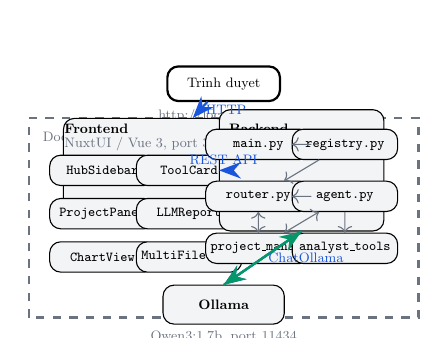
\begin{tikzpicture}[
  scale=0.55, transform shape,
  node distance=1.2cm,
  every node/.style={font=\small},
  block/.style={draw, rounded corners, minimum width=2.8cm, minimum height=0.9cm,
                text width=2.6cm, align=center, fill=white},
  service/.style={draw, rounded corners, minimum width=2.4cm, minimum height=0.7cm,
                  text width=2.2cm, align=center, fill=codebg, font=\small\ttfamily},
  label/.style={font=\small\bfseries\color{graytext}},
  arrow/.style={-{Stealth[scale=1.2]}, thick, color=primary},
  darrow/.style={-{Stealth[scale=1.2]}, thick, color=secondary},
]

% Docker boundary
\draw[dashed, thick, color=graytext] (-4.5,-0.6) rectangle (4.5,4.0);
\node[anchor=north west, font=\small\color{graytext}] at (-4.3,3.8) {Docker Compose};

% Browser
\node[draw, rounded corners, fill=white, minimum width=2.6cm, minimum height=0.8cm, thick] (browser) at (0,4.8) {Trinh duyet};
\node[font=\small\color{graytext}, below=0.05cm of browser] {http://localhost:3000};

% Frontend
\node[draw, rounded corners, fill=codebg, minimum width=3.8cm, minimum height=2.4cm,
      text width=3.5cm, align=center] (frontend) at (-1.8,2.8) {};
\node[anchor=north west] at (-3.8,4.0) {\textbf{Frontend}};
\node[font=\small\color{graytext}, anchor=north west] at (-3.8,3.7) {NuxtUI / Vue 3, port 3000};
\node[service] (sidebar) at (-2.8,2.8) {HubSidebar};
\node[service] (toolcard) at (-0.8,2.8) {ToolCard};
\node[service] (ppanel) at (-2.8,1.8) {ProjectPanel};
\node[service] (report) at (-0.8,1.8) {LLMReport};
\node[service] (chart) at (-2.8,0.8) {ChartView};
\node[service] (upload) at (-0.8,0.8) {MultiFileUpload};

% Backend
\node[draw, rounded corners, fill=codebg, minimum width=3.8cm, minimum height=2.8cm,
      text width=3.5cm, align=center] (backend) at (1.8,2.8) {};
\node[anchor=north west] at (0,4.0) {\textbf{Backend}};
\node[font=\small\color{graytext}, anchor=north west] at (0,3.7) {FastAPI, port 8000};
\node[service] (main) at (0.8,3.4) {main.py};
\node[service] (registry) at (2.8,3.4) {registry.py};
\node[service] (router) at (0.8,2.2) {router.py};
\node[service] (agent) at (2.8,2.2) {agent.py};
\node[service] (pmgr) at (0.8,1.0) {project\_manager};
\node[service] (tools) at (2.8,1.0) {analyst\_tools};

% Ollama
\node[draw, rounded corners, fill=codebg, minimum width=2.8cm, minimum height=0.9cm] (ollama) at (0,-0.3) {};
\node[font=\small\bfseries] at (0,-0.3) {Ollama};
\node[font=\small\color{graytext}, below=0.02cm of ollama] {Qwen3:1.7b, port 11434};

% Arrows
\draw[arrow] (browser) -- node[right, font=\small] {HTTP} (frontend);
\draw[arrow] (frontend.east) -- node[above, font=\small] {REST API} (backend.west);
\draw[arrow] (backend.south) -- node[right, font=\small] {ChatOllama} (ollama.north);
\draw[darrow] (backend.south) -- (ollama.north);
\draw[darrow] (ollama.north) -- (backend.south);

% Internal backend arrows
\draw[->, thin, color=graytext] (main) -- (registry);
\draw[->, thin, color=graytext] (registry) -- (router);
\draw[->, thin, color=graytext] (router) -- (agent);
\draw[->, thin, color=graytext] (agent) -- (tools);
\draw[<->, thin, color=graytext] (router) -- (pmgr);
\draw[<->, thin, color=graytext] (agent) -- (pmgr);

\end{tikzpicture}
\end{center}

\subsection{Luong du lieu (Data Flow)}

Quy trinh xu ly mot yeu cau phan tich du lieu:

\begin{enumerate}
  \item Nguoi dung truy cap \url{http://localhost:3000}, Frontend goi
        \texttt{GET /api/tools} de lay danh sach tool.
  \item Nguoi dung chon \texttt{Data Analytics}, Frontend hien thi ProjectPanel.
  \item Nguoi dung tao du an (\texttt{POST /project/create}).
  \item Nguoi dung tai file CSV (\texttt{POST /project/\{id\}/upload}).
        Backend luu DataFrame vao bo nho (ProjectManager).
  \item Nguoi dung nhap cau hoi va nhan ``Analyze''.
        Frontend goi \texttt{POST /project/\{id\}/analyze}.
  \item Backend tao LangChain agent (ChatOllama + 6 tools).
  \item Agent thuc hien ReAct loop: goi Ollama, chon tool, nhan Observation,
        lap lai cho den khi co ket qua.
  \item Agent tra ve bao cao (text) + bieu do (Plotly JSON).
  \item Frontend hien thi bao cao qua LLMReport va bieu do qua ChartView
        (ECharts).
\end{enumerate}

% ============================================================
%  4. PLUGIN REGISTRY
% ============================================================
\section{Plugin Registry}

\subsection{Co che \texttt{@register\_tool()}}

Tool Hub cho phep dang ky cong cu moi bang mot Python decorator. File
\texttt{backend/app/core/registry.py} dinh nghia co che nay:

\lstinputlisting[style=py]{tool-hub/backend/app/core/registry.py}

Trong do:
\begin{itemize}
  \item \texttt{\_tool\_registry} --- dictionary luu tru metadata cac tool.
  \item \texttt{@register\_tool(name, description, icon, router)} --- decorator
        gan nhan cho ham khoi tao tool.
  \item \texttt{discover\_tools()} --- tu dong quet cac module trong
        \texttt{app.tools} bang \texttt{pkgutil.iter\_modules}.
  \item \texttt{get\_all\_tools()} --- tra ve danh sach tool cho frontend.
  \item \texttt{get\_tool\_router(name)} --- tra ve router module cua tool.
\end{itemize}

Khi \texttt{app.tools} duoc import, \texttt{discover\_tools()} tu dong chay.
Moi tool package co mot file \texttt{router.py} dinh nghia APIRouter rieng.

\subsection{Cach them tool moi}

De them mot tool moi, chi can:

\begin{enumerate}
  \item Tao thu muc \texttt{backend/app/tools/<ten-tool>/}.
  \item Tao file \texttt{\_\_init\_\_.py} (rong).
  \item Tao file \texttt{router.py} voi noi dung:
\end{enumerate}

\lstinputlisting[style=py]{tool-hub/backend/app/tools/tool_template/router.py}

Sau do khoi dong lai backend, tool moi xuat hien trong danh sach
\texttt{GET /api/tools} va tren HubSidebar.

% ============================================================
%  5. BACKEND --- DATA ANALYTICS TOOL
% ============================================================
\section{Backend --- Data Analytics Tool}

\subsection{API Endpoints}

Tool Data Analytics cung cap 9 endpoint REST API trong
\texttt{router.py}:

\begin{tabularx}{\textwidth}{lXl}
\toprule
\bfseries Method & \bfseries Path & \bfseries Chuc nang \\
\midrule
POST & \texttt{/api/tools/data-analytics/upload}
      & Tai file CSV don, tra ve file\_id + preview \\
POST & \texttt{/api/tools/data-analytics/analyze}
      & Phan tich file don (backward compat) \\
POST & \texttt{/api/tools/data-analytics/project/create}
      & Tao du an moi (name + description) \\
GET  & \texttt{/api/tools/data-analytics/projects}
      & Danh sach tat ca du an \\
POST & \texttt{/api/tools/data-analytics/project/\{id\}/upload}
      & Tai CSV vao du an \\
GET  & \texttt{/api/tools/data-analytics/project/\{id\}}
      & Chi tiet du an (cac bang) \\
DELETE & \texttt{/api/tools/data-analytics/project/\{id\}}
      & Xoa du an \\
DELETE & \texttt{/api/tools/data-analytics/project/\{id\}/table/\{name\}}
      & Xoa bang khoi du an \\
POST & \texttt{/api/tools/data-analytics/project/\{id\}/analyze}
      & Phan tich toan bo du an (nhieu bang) \\
\bottomrule
\end{tabularx}

Gioi han upload: 50 MB (cau hinh trong \texttt{config.py}).

\subsection{Cau hinh (config.py)}

\lstinputlisting[style=py]{tool-hub/backend/app/config.py}

\subsection{Project Manager}

\texttt{project\_manager.py} dinh nghia hai lop chinh:

\begin{itemize}
  \item \textbf{Project}: Luu tru project\_id (UUID), name, description,
        tables dict (name $\rightarrow$ DataFrame), table\_order list.
        Cac phuong thuc: \texttt{add\_table} (co dedup), \texttt{remove\_table},
        \texttt{get\_schema\_summary}, \texttt{get\_context\_for\_agent}.
  \item \textbf{ProjectManager}: Singleton. Cac phuong thuc:
        \texttt{create\_project}, \texttt{get\_project},
        \texttt{delete\_project}, \texttt{list\_projects}.
\end{itemize}

Du lieu project duoc luu trong bo nho (RAM), se mat khi restart backend.
Co the mo rong bang SQLite trong tuong lai.

\subsection{Pydantic Schemas (schemas.py)}

Cac model Request/Response:

\begin{itemize}
  \item \texttt{UploadResponse}: file\_id, filename, columns, rows, preview
  \item \texttt{AnalyzeRequest}: question, file\_id
  \item \texttt{AnalyzeResponse}: stats, charts, report
  \item \texttt{CreateProjectRequest}: name, description
  \item \texttt{ProjectResponse}: project\_id, name, description, tables,
        table\_count
  \item \texttt{ProjectAnalyzeRequest}: question
  \item \texttt{ProjectAnalyzeResponse}: project\_id, tables\_context, report
\end{itemize}

% ============================================================
%  6. AGENT LANGCHAIN
% ============================================================
\section{Agent LangChain}

\subsection{Cach thuc hoat dong}

Agent duoc tao trong \texttt{agent/analyst.py} bang ham
\texttt{create\_project\_agent(project)}:

\begin{enumerate}
  \item Tao \texttt{ChatOllama} LLM (model tu \texttt{config.py}, temperature 0.3).
        \textbf{Luu y}: Su dung \texttt{langchain-ollama.ChatOllama} (khong phai
        \texttt{langchain\_community.llms.Ollama}) vi \texttt{ChatOllama} ho tro
        \texttt{.bind\_tools()}.
  \item Dinh dang \texttt{SYSTEM\_PROMPT} voi project context (ten bang,
        schema, so dong).
  \item Dinh nghia 6 tool function (xem ben duoi).
  \item Tao agent bang \texttt{create\_agent()} (LangGraph-based API,
        tra ve \texttt{CompiledStateGraph}).
  \item Goi agent voi \texttt{agent.invoke(\{"input": question\})}.
  \item Ket qua tra ve trong \texttt{result["messages"][-1].content}
        (khong phai \texttt{result["output"]}).
\end{enumerate}

\subsection{Sau cong cu (tools) cua agent}

\begin{enumerate}
  \item \textbf{list\_tables()}
        \begin{itemize}
          \item Tra ve danh sach ten bang trong project.
          \item Input: Khong co.
          \item Output: \texttt{"Tables: [sales\_2024, employees, ...]"}
        \end{itemize}

  \item \textbf{get\_table\_schema(table\_name)}
        \begin{itemize}
          \item Tra ve ten cot, kieu du lieu, va 3 dong mau.
          \item Input: \texttt{table\_name: str}
          \item Output: \texttt{"Column 'month' (object), 'revenue' (int64), ..."}
        \end{itemize}

  \item \textbf{get\_statistics(table\_name)}
        \begin{itemize}
          \item Thong ke co ban: so dong, so cot, missing values,
                mo ta so hoc (tu \texttt{df.describe()}).
          \item Goi \texttt{analyst\_tools/statistics.py}.
        \end{itemize}

  \item \textbf{query\_table(table\_name, query)}
        \begin{itemize}
          \item Truy van du lieu bang keyword (max, min, average, count,
                loc, Viet, Anh).
          \item Goi \texttt{analyst\_tools/query\_data.py}.
        \end{itemize}

  \item \textbf{join\_tables(table\_1, table\_2, on\_column)}
        \begin{itemize}
          \item Ghep hai bang theo cot (inner join).
          \item Bang ket qua duoc luu tam bang ten \texttt{"joined\_<table1>\_<table2>"}.
        \end{itemize}

  \item \textbf{generate\_chart(table\_name, chart\_type, x\_column,
        y\_column)}
        \begin{itemize}
          \item Ve bieu do bang Plotly Express.
          \item Ho tro: line, bar, scatter, histogram, heatmap (correlation).
          \item Tu dong phat hien loai bieu do neu \texttt{chart\_type="auto"}.
          \item Goi \texttt{analyst\_tools/chart\_generator.py}.
          \item Tra ve Plotly JSON de frontend render bang ECharts.
        \end{itemize}
\end{enumerate}

\subsection{System Prompt}

\texttt{agent/prompts.py} chua system prompt dai huong dan agent:

\begin{itemize}
  \item Su dung ReAct format: Thought / Action / Action Input /
        Observation / Final Answer.
  \item Tra loi bang cung ngon ngu voi nguoi dung (tieng Viet hoac tieng Anh).
  \item Khi can ve bieu do, luon goi \texttt{generate\_chart}.
  \item Khi can so sanh nhieu bang, su dung \texttt{join\_tables} truoc.
  \item Khong duoc tu y tao du lieu, chi phan tich du lieu co san.
\end{itemize}

% ============================================================
%  7. FRONTEND --- NUUI COMPONENTS
% ============================================================
\section{Frontend --- NuxtUI Components}

\subsection{Cau truc trang}

Frontend su dung NuxtUI (Vue 3) voi layout mac dinh gom:
\begin{itemize}
  \item \textbf{layouts/default.vue}: Sidebar ben trai + main content.
  \item \textbf{pages/index.vue}: Trang chu --- hien thi danh sach tool
        (\texttt{HubToolCard}).
  \item \textbf{pages/tools/data-analytics.vue}: Trang Data Analytics ---
        bo cuc 2 panel.
\end{itemize}

\subsection{7 Components Data Analytics}

\begin{tabularx}{\textwidth}{lX}
\toprule
\bfseries Component & \bfseries Chuc nang \\
\midrule
\texttt{ProjectPanel.vue}
& Danh sach du an, tao du an moi, chon du an \\
\texttt{TableList.vue}
& Danh sach bang trong du an, xoa bang (nut do khong confirm) \\
\texttt{MultiFileUpload.vue}
& Tai nhieu CSV (drag-drop), kiem tra 50MB, progress bar \\
\texttt{FileUpload.vue}
& Tai file don (backward compat), phan tich nhanh \\
\texttt{ChartView.vue}
& Render bieu do ECharts tu Plotly JSON \\
\texttt{StatsTable.vue}
& Hien thi thong ke (so dong, cot, missing, describe) \\
\texttt{LLMReport.vue}
& Hien thi bao cao AI \\
\bottomrule
\end{tabularx}

\subsection{API Client (useApi.ts)}

\lstinputlisting[style=ts]{tool-hub/frontend/composables/useApi.ts}

\subsection{Data Analytics Page (data-analytics.vue)}

Trang chinh bo cuc 2 panel:
\begin{itemize}
  \item \textbf{Panel trai} (288px co dinh): ProjectPanel + TableList.
  \item \textbf{Panel phai}: MultiFileUpload, o nhap cau hoi, nut
        ``Analyze Project'', LLMReport.
\end{itemize}

Tinh nang dac biet:
\begin{itemize}
  \item Nut ``Analyze'' bi disable khi cau hoi rong.
  \item Label nut dong thay doi: ``Analyzing...'' khi dang xu ly.
  \item \texttt{AbortController} voi 10-phut timeout tranh loading vo han.
\end{itemize}

% ============================================================
%  8. OLLAMA INTEGRATION
% ============================================================
\section{Ollama Integration}

\subsection{Docker Image}

\texttt{ollama/Dockerfile} su dung image chinh thuc \texttt{ollama/ollama} va
them entrypoint tuy chinh:

\lstinputlisting[style=bash]{tool-hub/ollama/Dockerfile}

\subsection{Entrypoint (auto-pull model)}

\lstinputlisting[style=bash]{tool-hub/ollama/entrypoint.sh}

Entrypoint thuc hien:
\begin{enumerate}
  \item Chay \texttt{ollama serve} trong background.
  \item Doi den khi server san sang (\texttt{until ollama list}).
  \item Kiem tra model da duoc pull chua; neu chua, chay
        \texttt{ollama pull \$OLLAMA\_DEFAULT\_MODEL}.
  \item Dua \texttt{ollama serve} len foreground bang \texttt{wait}.
\end{enumerate}

\subsection{Cau hinh model}

Model mac dinh: \texttt{qwen3:1.7b} (1.4 GB). Co the thay bang
\texttt{qwen3:4b} hoac model khac qua bien moi truong
\texttt{OLLAMA\_DEFAULT\_MODEL}. Dieu nay duoc cau hinh trong
\texttt{docker-compose.yml}:

\begin{lstlisting}[style=bash, language={}]
services:
  ollama:
    build: ./ollama
    environment:
      - OLLAMA_DEFAULT_MODEL=qwen3:1.7b
\end{lstlisting}

\subsection{CPU vs GPU}

May chu hien tai su dung CPU (AMD Lucienne, khong co NVIDIA GPU).
Thoi gian inference cho qwen3:1.7b khoang 6.5 phut cho mot yeu cau agent.
Khi co GPU, co the them \texttt{deploy.resources} de su dung CUDA.

% ============================================================
%  9. DEPLOYMENT
% ============================================================
\section{Deployment}

\subsection{Docker Compose (Local)}

\texttt{docker-compose.yml} dinh nghia 3 services:

\begin{lstlisting}[style=bash, language={}]
services:
  ollama:
    build: ./ollama
    ports: ["11434:11434"]
    volumes: [ollama_data:/root/.ollama]
    environment:
      - OLLAMA_DEFAULT_MODEL=qwen3:1.7b

  backend:
    build: ./backend
    ports: ["8000:8000"]
    depends_on: [ollama]
    volumes: [./backend:/app]        # hot-reload khi dev
    environment:
      - MODEL_NAME=qwen3:1.7b
      - OLLAMA_HOST=http://ollama:11434
      - CORS_ORIGINS=http://localhost:3000

  frontend:
    build: ./frontend
    ports: ["3000:3000"]
    depends_on: [backend]
    environment:
      - API_BASE_URL=http://localhost:8000

volumes:
  ollama_data:
\end{lstlisting}

Lenh chay:
\begin{lstlisting}[style=bash, language={}]
docker compose up --build -d
docker compose logs -f
\end{lstlisting}

\subsection{Docker Compose (Cloud)}

\begin{tabularx}{\textwidth}{lX}
\toprule
\bfseries Dich vu & \bfseries Mo ta \\
\midrule
\textbf{Vercel} & Frontend (NuxtUI). Build: \texttt{cd frontend \&\&}
                  \texttt{npm install \&\& npm run build}. Output:
                  \texttt{frontend/.output/public}. \\
\textbf{Render}  & Backend (FastAPI). Build: \texttt{pip install -r
                  backend/requirements.txt}. Start: \texttt{uvicorn
                  app.main:app --host 0.0.0.0 --port 8000}. \\
\textbf{Ollama}  & Chay local hoac tren VPS rieng. Khong the deploy len
                  serverless. \\
\bottomrule
\end{tabularx}

\subsection{Bien moi truong}

\begin{tabularx}{\textwidth}{lXl}
\toprule
\bfseries Bien & \bfseries Gia tri mac dinh & \bfseries Dich vu \\
\midrule
\texttt{MODEL\_NAME} & \texttt{qwen3:1.7b} & Backend \\
\texttt{OLLAMA\_HOST} & \texttt{http://ollama:11434} & Backend \\
\texttt{CORS\_ORIGINS} & \texttt{http://localhost:3000} & Backend \\
\texttt{UPLOAD\_DIR} & \texttt{backend/app/uploads} & Backend \\
\texttt{MAX\_UPLOAD\_MB} & \texttt{50} & Backend \\
\texttt{API\_BASE\_URL} & \texttt{http://localhost:8000} & Frontend \\
\texttt{OLLAMA\_DEFAULT\_MODEL} & \texttt{qwen3:1.7b} & Ollama \\
\bottomrule
\end{tabularx}

% ============================================================
%  10. HUONG DAN CHAY
% ============================================================
\section{Huong dan chay chuong trinh}

\subsection{Cach 1: Docker Compose (khuyen nghi)}

Day la cach don gian nhat, khong can cai dat Python hay Node.

\begin{enumerate}
  \item Cai dat Docker va Docker Compose:
\begin{lstlisting}[style=bash, language={}]
sudo apt install docker.io docker-compose-v2
sudo systemctl start docker
\end{lstlisting}

  \item Chay toan bo he thong:
\begin{lstlisting}[style=bash, language={}]
cd tool-hub
docker compose up --build -d
\end{lstlisting}

  \item Kiem tra trang thai:
\begin{lstlisting}[style=bash, language={}]
docker compose ps
\end{lstlisting}
        Ca 3 services phai o trang thai \texttt{Up}.

  \item Truy cap \url{http://localhost:3000}.

  \item Xem log:
\begin{lstlisting}[style=bash, language={}]
docker compose logs -f backend
docker compose logs -f ollama
\end{lstlisting}

  \item Tat he thong:
\begin{lstlisting}[style=bash, language={}]
docker compose down
\end{lstlisting}
        Them \texttt{-v} neu muon xoa ca volumes (mat model Ollama).
\end{enumerate}

\subsection{Cach 2: Thu cong (Local dev)}

\subsubsection{Buoc 1: Ollama}

\begin{lstlisting}[style=bash, language={}]
# Cai dat Ollama: https://ollama.com
ollama serve &
ollama pull qwen3:1.7b
\end{lstlisting}

\subsubsection{Buoc 2: Backend}

\begin{lstlisting}[style=bash, language={}]
cd tool-hub/backend
python3 -m venv .venv
source .venv/bin/activate
pip install -r requirements.txt
uvicorn app.main:app --host 0.0.0.0 --port 8000 --reload
\end{lstlisting}

\subsubsection{Buoc 3: Frontend}

\begin{lstlisting}[style=bash, language={}]
cd tool-hub/frontend
npm install
npm run dev
\end{lstlisting}

\subsubsection{Buoc 4: Su dung}

\begin{enumerate}
  \item Mo \url{http://localhost:3000}.
  \item Tao project moi (``Create Project'').
  \item Tai file CSV (keo tha hoac click).
  \item Nhap cau hoi va nhan ``Analyze Project''.
  \item Doi agent xu ly (khoang 6.5 phut tren CPU).
\end{enumerate}

\subsection{Cach 3: Cloud (Vercel + Render)}

\begin{enumerate}
  \item Push code len GitHub.
  \item Tren Render: Tao Web Service, tro den \texttt{backend/},
        build command \texttt{pip install -r requirements.txt},
        start command \texttt{uvicorn app.main:app --host 0.0.0.0 --port 8000}.
  \item Tren Vercel: Import project, framework la NuxtJS,
        root directory la \texttt{frontend/}.
  \item Cau hinh rewrite trong \texttt{vercel.json} de proxy
        \texttt{/api/*} den Render.
  \item Ollama can chay rieng (VPS hoac local).
\end{enumerate}

\subsection{Xu ly loi thuong gap}

\begin{tabularx}{\textwidth}{lX}
\toprule
\bfseries Loi & \bfseries Cach xu ly \\
\midrule
Backend khong ket noi duoc Ollama
& Kiem tra \texttt{OLLAMA\_HOST} trong \texttt{docker-compose.yml} \\
Model chua duoc pull
& \texttt{docker compose exec ollama ollama pull qwen3:1.7b} \\
Frontend loi CORS
& Kiem tra \texttt{CORS\_ORIGINS} bang voi frontend URL \\
Upload that bai (file > 50MB)
& Tang \texttt{MAX\_UPLOAD\_MB} trong \texttt{config.py} \\
Agent tra ve loi
& Kiem tra log backend: \texttt{docker compose logs backend} \\
YAML loi khi docker compose
& Kiem tra khoang trang, xoa ky tu dac biet trong .yml \\
\bottomrule
\end{tabularx}

% ============================================================
%  11. KET LUAN
% ============================================================
\section{Ket luan}

\subsection{Da hoan thanh}

\begin{itemize}
  \item Tool Hub voi kien truc hybrid (FastAPI + NuxtUI + LangChain + Ollama).
  \item Co che plugin \texttt{@register\_tool()} de dang mo rong.
  \item Data Analytics Tool voi 6 cong tu phan tich du lieu.
  \item Ho tro da bang (multi-table): agent co the lam viec voi nhieu file
        CSV trong cung mot du an.
  \item Docker Compose 3 services chay on dinh.
  \item Hoi dap song ngu Viet-Anh.
  \item Bieu do Plotly $\rightarrow$ ECharts.
  \item Upload 50 MB.
\end{itemize}

\subsection{Huong phat trien}

\begin{tabularx}{\textwidth}{lX}
\toprule
\bfseries Huong & \bfseries Mo ta \\
\midrule
SQLite persistence
& Luu project vao database thay vi in-memory \\
GPU acceleration
& Them CUDA de tang toc inference \\
Multi-model
& Cho phep chon model (Qwen, Llama, Mistral) \\
Them tool moi
& Phan tich PDF, Web scraping, SQL query, ... \\
Dashboard
& Trang tong quan voi nhieu bieu do cung luc \\
Authentication
& Them dang nhap / phan quyen \\
\bottomrule
\end{tabularx}

\subsection{Thong tin lien quan}

\begin{tabularx}{\textwidth}{lX}
\toprule
\bfseries Tai lieu & \bfseries Link \\
\midrule
FastAPI & \url{https://fastapi.tiangolo.com} \\
NuxtUI & \url{https://ui.nuxt.com} \\
LangChain & \url{https://python.langchain.com} \\
Ollama & \url{https://ollama.com} \\
Plotly & \url{https://plotly.com/python} \\
ECharts & \url{https://echarts.apache.org} \\
Docker Compose & \url{https://docs.docker.com/compose} \\
\bottomrule
\end{tabularx}

\end{document}
